% ============================================================================
% Staged Calibration of Tensor-Basis Turbulence Closures:
% Transient Realizability Dynamics in Nested Subspaces
% ============================================================================
\documentclass[preprint,aps,prb,longbibliography,superscriptaddress]{revtex4-2}

\usepackage{amsmath,amssymb,amsthm}
\usepackage{booktabs}
\usepackage{graphicx}
\usepackage{siunitx}
\usepackage{tikz}
\usetikzlibrary{arrows.meta,positioning,calc}
\usepackage{xcolor}
\usepackage{hyperref}
\usepackage{multirow}

\hypersetup{
  colorlinks=true,
  linkcolor=blue!60!black,
  citecolor=blue!60!black,
  urlcolor=blue!60!black,
}

% --- Custom commands ---
\newcommand{\bx}{\mathbf{x}}
\newcommand{\bU}{\mathbf{U}}
\newcommand{\bI}{\mathbf{I}}
\newcommand{\Tr}{\operatorname{Tr}}
\newcommand{\dR}{\delta_R}
\newcommand{\fsec}{f_{\text{sec}}}
\newcommand{\tref}{\tau_{\text{ref}}}

\newcommand{\id}{\mathbb{I}}

\begin{document}

% ============================================================================
\title{Staged Calibration of Tensor-Basis Turbulence Closures:\\
Transient Realizability Dynamics in Nested Subspaces}

\author{Okuhle Madondo}
\affiliation{Rosetta Technologies}
\email{okuhlemadondo@users.noreply.github.com}

\date{\today}

% ============================================================================
\begin{abstract}
In a convex, constant-coefficient, \emph{a~priori} calibration of a four-term
Pope tensor basis on a synthetic square duct benchmark ($\mathrm{Re}_\tau = 300$),
we investigate whether staging calibration through intermediate subspaces
offers measurable advantages over direct joint calibration or a cold start.
Because zero-padding preserves predictions identically ($\delta_R \equiv 0$),
the deployed Stratum~2 model in the staged protocol inherits the full $5.64\%$
realizability violation of the intermediate scaffold at deployment (peaking at
$5.90\%$ during repair due to Adam's cold-update sign-step transient), whereas direct
calibration produces a transient excursion peaking at $2.00\%$ violation
(accompanied by a $1.68\times$ loss rebound), and an un-staged cold start
($\theta = \mathbf{0}$) reaches the identical minimizer with a peak violation of
only $1.22\%$.

Through an extensive suite of pre-registered controls, we isolate the physical
and numerical mechanisms governing these dynamics. In a matched-loss restart control
at step~18 (matching Path~A's hop loss $\num{4.73e-9}$), resetting momentum yields
a post-restart peak violation of $1.74\%$ with a $3.12\times$ loss rebound, confirming
that travel distance across the ill-conditioned landscape is the dominant driver of
realizability excursions, while continuous mid-descent momentum provides an incremental
amplification of $+0.26\%$. Setting $\beta_1 = 0$ in Adam reduces peak violation from
$2.00\%$ to $1.30\%$ across extended horizons, while convergent plain gradient descent
traverses unrealizable states at $6.25\%$. Furthermore, we demonstrate that
per-coordinate Adam on a unit-normalized basis preserves exact scale invariance to
machine precision (relative loss discrepancy $< \num{1e-14}$, parameter difference
$< \num{3e-17}$).

In this convex setting, neither staged nor warm-started calibration confers an
advantage in convergence speed, endpoint accuracy, or peak violation over a
cold start. We formalize this configuration space as a \emph{Stratified Design
Atlas} and delineate the necessary conditions---non-convex losses, coupled
Navier--Stokes evaluation, and non-nested basis edits---under which geometric
transport and path-dependence become non-trivial.
\end{abstract}

\maketitle

% ============================================================================
\section{Introduction}\label{sec:intro}
% ============================================================================

Turbulence closure modeling for Reynolds-Averaged Navier--Stokes (RANS)
equations remains one of the foundational open challenges in computational
fluid dynamics. The Reynolds stress tensor
$\tau_{ij} = \overline{u_i' u_j'}$ represents the statistical effect of
turbulent fluctuations on the mean momentum field. For decades, practical
engineering CFD has relied on linear eddy-viscosity models governed by the
Boussinesq hypothesis~\cite{Boussinesq1877}:
\begin{equation}\label{eq:boussinesq}
  \tau_{ij} - \tfrac{2}{3}k\,\delta_{ij} = -2\,\nu_t\, S_{ij}\,,
\end{equation}
where $k$ is the turbulent kinetic energy, $\nu_t$ is the scalar eddy
viscosity, and $S_{ij} = \tfrac{1}{2}(\partial_j U_i + \partial_i U_j)$ is
the mean strain rate tensor.

While computationally robust, the Boussinesq hypothesis fails qualitatively in
complex strain fields---most notoriously in non-circular duct flows, where
turbulent secondary motion of the second kind~\cite{Prandtl1926} is driven
predominantly by Reynolds normal stress anisotropy
$(\tau_{yy} - \tau_{zz})$ and cross-stream shear stress
$\tau_{yz}$~\cite{Speziale1987}. Linear models produce secondary vorticity
forcing that is anti-aligned with the physical forcing pattern, a classical
result established by Speziale~\cite{Speziale1987}.

To overcome these deficiencies, higher-order non-linear eddy viscosity models
\cite{Pope1975,Pope2000,Craft1996,Wallin2000} expand the anisotropy tensor in a basis of
symmetric, traceless tensors formed from strain and rotation rates. Modern
data-driven and automated model discovery frameworks~\cite{Duraisamy2019,Ling2016,Weatheritt2016,Schmelzer2020,Parish2016,Wu2018,Kochkov2021,List2022}
face a fundamental dilemma when navigating structural model hierarchies:
\begin{itemize}
  \item \textit{Cold-start cost.} Re-optimizing all continuous parameters from
    scratch ($\theta = \mathbf{0}$) each time a structural modification is made
    (adding or swapping tensor basis terms) discards prior calibration work.
  \item \textit{Warm-starting risks.} In deep learning, function-preserving model
    growth techniques such as Net2Net~\cite{Chen2016} and network morphisms~\cite{Wei2016}
    guarantee that newly introduced capacities initially leave predictions unchanged.
    However, warm-starting neural network training frequently underperforms cold
    starts due to momentum carry-over, optimization basins, and catastrophic forgetting~\cite{Ash2020,Hinton2015,Frankle2018,Draxler2018,Garipov2018,Ainsworth2022,Bengio2009}.
    In turbulence closure calibration, initializing new coefficients to zero
    preserves prior predictions identically by construction ($\delta_R \equiv 0$),
    but the subsequent optimization trajectory may venture into unrealizable parameter
    regimes where the Reynolds stress tensor violates positive semi-definiteness
    \cite{Schumann1977,Lumley1978}.
\end{itemize}

\subsection{Approach and Scope}\label{sec:scope}

We formalize the configuration space of candidate closures as a
\emph{Stratified Design Atlas}:
\begin{equation}\label{eq:atlas}
  \mathcal{A} = \bigl(\{\Theta_s\},\, L,\, \{T_e\}\bigr)\,,
\end{equation}
where $\Theta_s$ are continuous parameter manifolds (strata) corresponding
to specific algebraic tensor bases, $L$ is the calibration loss functional
penalizing realizability violations, and $T_e: \Theta_s \to \Theta_{s'}$ are
transport mappings carrying calibrated states across structural transitions.

In the simplest instantiation studied here---nested constant-coefficient Pope
subspaces with a convex quadratic task loss---the parameter spaces are
$\Theta_s = \mathbb{R}^{d_s}$, the transport maps $T_e$ are zero-padding
embeddings, realization drift vanishes identically ($\dR \equiv 0$ by
construction), and the global minimizer is unique. The geometric vocabulary
names structure that is algebraically trivial in this setting; its value lies
in establishing a rigorous, fully characterized baseline against which future
extensions to non-nested edits and non-convex losses (Sec.~\ref{sec:discussion})
can be evaluated.

The objective of this paper is a controlled \emph{a~priori} investigation of
the \emph{transient optimization dynamics} of warm-started vs.\ cold-started
calibrations under realizability constraints:
\begin{enumerate}
  \item We quantify the stress-representability gap between linear and
    quadratic Pope strata, recovering the classical result~\cite{Speziale1987}
    that linear closures produce anti-aligned secondary vorticity forcing.
  \item We analyze the dynamics of staged calibration ($\mathcal{M}_0 \to
    \mathcal{M}_1 \to \mathcal{M}_2$), direct warm-starting ($\mathcal{M}_0 \to
    \mathcal{M}_2$), and cold-starting ($\mathcal{M}_2$ from $\theta = \mathbf{0}$).
    Because $\delta_R \equiv 0$, staging inherits the intermediate scaffold's
    $5.64\%$ violation upon deployment, while cold-starting achieves the lowest
    peak violation ($1.22\%$) throughout the descent.
  \item Through a suite of optimizer controls (convergent plain GD, Adam with
    $\beta_1 = 0$, and step-size rescalings), we isolate the mechanism of
    transient excursions: travel distance per step and adaptive coordinate
    scaling, rather than Gram matrix ill-conditioning.
\end{enumerate}

% ============================================================================
\section{Mathematical Formulation}\label{sec:math}
% ============================================================================

\subsection{Governing Equations and Secondary Flow Mechanics}
\label{sec:governing}

Consider steady, incompressible turbulent flow through a straight square duct
of width $h$ aligned with the $x$-axis. The mean velocity field is
$\bU = (U(y,z),\, V(y,z),\, W(y,z))$, which is $x$-independent but
three-dimensional: $\partial U/\partial y$, $\partial U/\partial z \neq 0$,
and secondary cross-plane velocities $(V,W)$ are nonzero.

The streamwise mean vorticity is defined as
\begin{equation}\label{eq:vorticity}
  \omega_x = \frac{\partial W}{\partial y} - \frac{\partial V}{\partial z}\,.
\end{equation}
In fully developed straight square duct flow ($\partial/\partial x \equiv 0$), the transport equation for $\omega_x$
reduces to
\begin{equation}\label{eq:vorticity_transport}
  V\frac{\partial \omega_x}{\partial y}
  + W\frac{\partial \omega_x}{\partial z}
  = \nu \nabla_{yz}^2 \omega_x + \fsec(\bx)\,,
\end{equation}
where the secondary vorticity driving force $\fsec$ is governed by spatial
derivatives of the Reynolds stress tensor:
\begin{equation}\label{eq:fsec}
  \fsec(\bx) =
  \underbrace{\frac{\partial^2}{\partial y\,\partial z}
    (\tau_{yy} - \tau_{zz})}_{\text{Normal stress anisotropy}}
  +\;
  \underbrace{\left(\frac{\partial^2}{\partial z^2}
    - \frac{\partial^2}{\partial y^2}\right)\tau_{yz}}_{\text{Cross-plane shear stress}}\,.
\end{equation}
Equation~(\ref{eq:vorticity_transport}) establishes $\fsec$ as the direct
source term generating streamwise secondary vortices.

\subsection{Tensor Integrity Basis and Nested Subspaces}
\label{sec:basis}

The symmetric mean strain rate tensor $S$ and anti-symmetric mean rotation rate
tensor $\Omega$ are defined by
\begin{equation}
  S_{ij} = \tfrac{1}{2}(\partial_j U_i + \partial_i U_j), \quad
  \Omega_{ij} = \tfrac{1}{2}(\partial_j U_i - \partial_i U_j)\,.
\end{equation}
Their dimensionless counterparts scale with the turbulent timescale
$\tau_t = 1/(C_\mu \omega)$.

Following Pope~\cite{Pope1975,Pope2000}, the deviatoric Reynolds stress anisotropy
$a_{ij} = \tau_{ij}/k - \tfrac{2}{3}\delta_{ij}$ can be expanded in a
complete integrity basis:
\begin{equation}\label{eq:pope_expansion}
  a_{ij} = \sum_{n=1}^{N} c_n\, T_{ij}^{(n)}\,,
\end{equation}
where we identify $c_n \equiv \theta_{n-1}$. In the square duct, the flow has
three-dimensional strain via $\partial U/\partial y$ and $\partial U/\partial z$.
We select four tensors from Pope's ten-term integrity basis to form three
nested subspaces with spatially constant coefficients $\theta \in \mathbb{R}^d$:

\paragraph{Stratum~0 ($\mathcal{M}_0$, Linear Boussinesq, $d_0 = 1$).}
\begin{equation}\label{eq:stratum0}
  \tau^{(0)}(\bx;\theta) = \tfrac{2}{3}k\,\id + \theta_0\, T^{(1)},
  \qquad
  T^{(1)} = -\frac{2k}{\omega}\, S\,,
\end{equation}
where $\theta_0 = C_\mu \approx 0.09$.

\paragraph{Stratum~1 ($\mathcal{M}_1$, Quadratic Pope, $d_1 = 3$).}
\begin{equation}\label{eq:stratum1}
  \tau^{(1)}(\bx;\theta) = \tfrac{2}{3}k\,\id
  + \theta_0\, T^{(1)}
  + \theta_1\, T^{(2)}
  + \theta_2\, T^{(3)}\,,
\end{equation}
with quadratic invariant tensors
\begin{equation}\label{eq:T2T3}
  T^{(2)} = \frac{k}{(C_\mu\omega)^2}
    \Bigl(S^2 - \tfrac{1}{3}\Tr(S^2)\,\id\Bigr),
  \quad
  T^{(3)} = \frac{k}{(C_\mu\omega)^2}
    \bigl(S\Omega - \Omega S\bigr).
\end{equation}

\paragraph{Stratum~2 ($\mathcal{M}_2$, Cubic Pope, $d_2 = 4$).}
\begin{equation}\label{eq:stratum2}
  \tau^{(2)}(\bx;\theta) = \tfrac{2}{3}k\,\id
  + \sum_{i=0}^{3} \theta_i\, T^{(i+1)}\,,
\end{equation}
incorporating the cubic tensor
\begin{equation}\label{eq:T4}
  T^{(4)} = \frac{k}{(C_\mu\omega)^3}
    \bigl(S^2\Omega - \Omega S^2\bigr).
\end{equation}

\subsection{Stress-Representability Metrics}
\label{sec:representability}

To quantify whether a subspace can represent secondary flow driving stresses,
we define two distinct metrics.

The \emph{stress-projection alignment} $\cos\phi_{\mathrm{sec}}$ measures
whether the secondary stress pattern $\tau_{\mathrm{sec}}$ (the
$(\tau_{yy}-\tau_{zz})$ and $\tau_{yz}$ components of $\tref$) lies in the
$L^2(\Omega)$ span of the basis tensors:
\begin{equation}\label{eq:controllability}
  \cos\phi_{\mathrm{sec}}(\mathcal{M}_s) =
  \frac{\langle \tau_{\mathrm{sec}},\;
        \mathrm{proj}_{\mathcal{M}_s}\tau_{\mathrm{sec}}
        \rangle_{L^2(\Omega)}}
       {\|\tau_{\mathrm{sec}}\|_{L^2}\;
        \|\mathrm{proj}_{\mathcal{M}_s}\tau_{\mathrm{sec}}\|_{L^2}}\,.
\end{equation}

The \emph{forcing correlation} $\rho$ measures the alignment of the secondary
vorticity forcing field $\fsec(\tau(\theta))$ produced by a specific model with
the reference forcing field $\fsec(\tref)$:
\begin{equation}\label{eq:rho}
  \rho(\theta) =
  \frac{\langle \fsec(\tau(\theta)),\;
        \fsec(\tref) \rangle_{L^2(\Omega)}}
       {\|\fsec(\tau(\theta))\|_{L^2}\;
        \|\fsec(\tref)\|_{L^2}}\,.
\end{equation}
These metrics measure fundamentally different quantities: $\cos\phi_{\mathrm{sec}}$
is a property of the subspace span (independent of $\theta$), while $\rho(\theta)$
evaluates the field-level vorticity forcing at a specific parameter state $\theta$
and involves second spatial derivatives.

\subsection{Zero-Padding Embeddings and Loss Landscape}
\label{sec:embedding}

For nested inclusions $\mathcal{M}_s \subset \mathcal{M}_{s'}$, the canonical
transport map is zero-padding:
\begin{equation}\label{eq:transport}
  T_e(\theta) = \bigl[\theta_0,\, \theta_1,\, \dotsc,\,
    \theta_{d_s-1},\,
    \underbrace{0,\, \dotsc,\, 0}_{d_{s'}-d_s}\bigr].
\end{equation}
Because the model is linear in $\theta$, zero-padding preserves predictions
identically: $\tau^{(s')}(T_e(\theta)) \equiv \tau^{(s)}(\theta)$ pointwise.
The realization drift vanishes identically by construction:
\begin{equation}\label{eq:drift}
  \dR = \frac{\|\tau^{(s')}(T_e(\theta)) - \tau^{(s)}(\theta)\|_{L^2}}
             {\|\tref\|_{L^2}} \equiv 0\,.
\end{equation}
This preservation property parallels functional preserving operations in neural
network growth techniques such as Net2Net~\cite{Chen2016} and network morphisms~\cite{Wei2016},
where newly introduced dimensions are zero-initialized to guarantee invariant
input--output predictions at transition.

The task loss is the integrated Frobenius discrepancy:
\begin{equation}\label{eq:task_loss}
  L_{\text{task}}(\theta) = \frac{1}{2}\int_\Omega
  \|\tau(\bx;\theta) - \tref(\bx)\|_F^2\,dA\,,
\end{equation}
which is quadratic with constant Hessian equal to the spatial Gram matrix:
\begin{equation}\label{eq:gram}
  G_{ij} = \int_\Omega \Tr\bigl(T^{(i)}(\bx)\, T^{(j)}(\bx)\bigr)\,dA\,.
\end{equation}

To penalize non-physical states, a realizability penalty is added:
\begin{equation}\label{eq:penalty}
  L(\theta) = L_{\text{task}}(\theta)
  + \lambda_{\mathrm{realiz}}
    \int_\Omega \max\!\bigl(0,\, -\lambda_{\min}(\tau(\bx;\theta))\bigr)^2\,dA\,,
\end{equation}
where $\lambda_{\min}$ is the smallest eigenvalue of the local stress tensor.
Because $\lambda_{\min}$ is a concave function of symmetric matrices,
$-\lambda_{\min}$ is convex. Its composition with the convex non-decreasing
function $\max(0,\cdot)^2$ is convex. Since $L_{\text{task}}$ is quadratic
convex, the full loss $L(\theta)$ is strictly convex when $G \succ 0$.
Consequently, all paths share a unique global minimizer; observed differences at
convergence reflect numerical optimization tolerances rather than separate
local basins.

We define the convergence diagnostic:
\begin{equation}\label{eq:CAB}
  C_{AB}
  = \frac{\|\tau^{(2)}(\theta_{2,A}^*) -
          \tau^{(2)}(\theta_{2,B}^*)\|_{L^2(\Omega)}}
         {\|\tref\|_{L^2(\Omega)}}\,,
\end{equation}
which measures how closely two optimization trajectories have approached the
shared minimizer.

% ============================================================================
\section{Experimental Setup}\label{sec:setup}
% ============================================================================

\subsection{Synthetic Benchmark}\label{sec:benchmark}

We discretized a square duct quadrant $(y,z) \in [0,h] \times [0,h]$ on a
$48 \times 48$ non-uniform grid clustered near the walls using hyperbolic
tangent stretching ($y_1^+ \approx 0.8$). Mean flow fields ($U, V, W, k, \omega$)
were synthesized from analytical profiles reproducing the qualitative secondary
vortex structure of DNS data at $\mathrm{Re}_\tau = 300$~\cite{Pinelli2010}.
The Reynolds number is a label characterizing the target flow regime and does
not enter the algebraic field synthesis.

The reference stress field $\tref$ is constructed synthetically:
\begin{equation}\label{eq:tref}
  \tref = \tfrac{2}{3}k\,\id + \sum_{n=1}^{4} c_n^{\mathrm{true}}\, T^{(n)}
  + \tau_{\mathrm{wall}}\,,
\end{equation}
with true coefficients $[c_1, c_2, c_3, c_4]^{\mathrm{true}} =
[0.090,\, 0.045,\, {-}0.035,\, 0.060]$ and an unmodeled wall stress perturbation
$\tau_{\mathrm{wall}} = 0.015\,(k/\omega^2)\sin(\pi y)\sin(\pi z)\,S^2$.

Due to this unmodeled perturbation, $\tref$ itself carries a slight realizability
violation of $1.56\%$ ($\min\lambda(\tref) = \num{-5.10e-5}$, corresponding to
$\num{-1.17e-3}\max(k)$). The perturbation ensures controlled misspecification:
no stratum can achieve zero loss. Because $\tref$ is constructed from the Pope
basis, $\cos\phi_{\mathrm{sec}}(\mathcal{M}_1) = 1.0$ follows by construction;
this study isolates numerical optimization dynamics rather than modeling
fidelity against physical DNS measurements.

\subsection{Traversal Protocols}\label{sec:protocols}

We evaluate three calibration protocols under a budget of $N = 220$ gradient
steps with baseline penalty $\lambda_{\mathrm{realiz}} = 150$:
\begin{itemize}
  \item \textit{Path~A (Staged warm-start):} 100 steps in Stratum~1
    ($\mathcal{M}_1$, $d=3$), followed by zero-padding $\theta_3 = 0$
    ($\delta_R \equiv 0$) and a fresh Adam optimizer ($m = v = 0$), then
    120 steps in Stratum~2 ($\mathcal{M}_2$, $d=4$) with all parameters free.
  \item \textit{Path~B (Direct warm-start):} 220 steps in Stratum~2,
    initialized from $T_e(\theta_0^*) = [0.089849,\, 0,\, 0,\, 0]$.
  \item \textit{Path~C (Cold start):} 220 steps in Stratum~2 from
    $\theta = [0,\, 0,\, 0,\, 0]$.
\end{itemize}

\emph{Terminology.} We designate Path~A's Stratum~1 iterates as the
\emph{scaffold} (in the sense of curriculum learning~\cite{Bengio2009}, discarded
upon transition) and its Stratum~2 iterates as \emph{deployed}. The \emph{violation fraction} is the percentage of grid
cells where $\lambda_{\min}(\tau) < -10^{-6}$. Relative to the peak turbulent
kinetic energy ($k_{\max} \approx 0.043$), this cutoff corresponds to a
non-dimensional tolerance $\lambda_{\min}/k_{\max} < -2.3\times 10^{-5}$.
Sweeping the threshold across orders of magnitude from $-10^{-7}$ to $-10^{-5}$
shifts Path~B's peak violation from $2.17\%$ to $1.04\%$ while preserving the
qualitative trajectory geometry, confirming that the transient excursions are
not an artifact of the specific numerical cutoff.

% ============================================================================
\section{Results}\label{sec:results}
% ============================================================================

\subsection{Stress-Representability and Boussinesq Failure}
\label{sec:representability_results}

\begin{table}[t]
\caption{Stress-representability and forcing alignment across strata. $\cos\phi_{\mathrm{sec}}$
  measures secondary stress representation in the basis span (Eq.~\ref{eq:controllability});
  $\rho(\theta^*)$ measures field-level forcing correlation (Eq.~\ref{eq:rho}).
  Because synthesized secondary velocities $V, W \neq 0$ produce weak
  strain anisotropy $S_{yy} - S_{zz} \neq 0$, $\cos\phi_{\mathrm{sec}}(\mathcal{M}_0)$ is small
  ($\num{1.15e-4}$) but not identically zero.}\label{tab:representability}
\begin{ruledtabular}
\begin{tabular}{lccc}
  Metric & Stratum~0 (Linear) & Stratum~1 (Quadratic) & Stratum~2 (Cubic) \\
  \midrule
  $\cos\phi_{\mathrm{sec}}$ (stress projection)
    & $\num{1.15e-4} \approx 0$ & $1.000$ & $1.000$ \\[3pt]
  $\rho(\theta^*)$ (forcing correlation)\footnotemark[1]
    & $-0.157$ & $+0.294$ & $+0.999$ \\[3pt]
  Reversed forcing fraction
    & $29.38\%$ & $20.36\%$ & $1.65\%$ \\
\end{tabular}
\end{ruledtabular}
\footnotetext[1]{$\rho(\theta^*)$ is the spatial correlation (Eq.~\ref{eq:rho}) between model-generated secondary flow forcing $\fsec(\tau(\theta^*))$ and reference forcing $\fsec(\tref)$ evaluated at the calibrated parameter state $\theta^*$. Unlike $\cos\phi_{\mathrm{sec}}$, which is a static property of the basis subspace span, $\rho(\theta^*)$ evaluates field derivatives of the instantiated closure. Note that Stratum-1 $\rho = +0.294$ is evaluated at the $\lambda_{\mathrm{realiz}}=150$-regularized scaffold iterate after 100 gradient steps, not the unconstrained Stratum-1 minimizer.}
\end{table}

Table~\ref{tab:representability} summarizes representability metrics for the
linear and quadratic strata. The stress projection alignment
$\cos\phi_{\mathrm{sec}}(\mathcal{M}_0) = \num{1.15e-4} \approx 0$ confirms
that the linear Boussinesq basis is nearly incapable of generating the required
stress anisotropy pattern. The value is not identically zero because the
evaluation field contains nonzero secondary velocities ($V,W \neq 0$), yielding
weak strain anisotropy $S_{yy} - S_{zz} \neq 0$.

At the calibrated parameter $\theta_0^* = 0.089849$, the linear model yields a
negative forcing correlation $\rho = -0.157$, with $29.38\%$ of the quadrant
exhibiting reversed secondary vorticity forcing. This reproduces Speziale's
classical result~\cite{Speziale1987}: linear eddy-viscosity models drive
secondary flow in the direction opposite to physical corner vortices.

\subsection{Gram Matrix Structure and Conditioning Decomposition}
\label{sec:gram_results}

\begin{table}[t]
\caption{Full spatial Gram matrix $G_{ij}$ (Eq.~\ref{eq:gram}) and its
  normalized correlation matrix $R_{ij} = G_{ij}/\sqrt{G_{ii}G_{jj}}$.
  The block-diagonal structure ($G_{ij} < 10^{-17}$ for $i \in \{1,2\}$,
  $j \in \{3,4\}$) is an algebraic identity: because $A$ and $B$ are polynomials
  in $S$, they commute ($[A,B] = 0$), so $\Tr(A[B,\Omega]) = \Tr([A,B]\Omega) = 0$.}\label{tab:gram}
\begin{ruledtabular}
\begin{tabular}{lcccc}
  & $T^{(1)}$ & $T^{(2)}$ & $T^{(3)}$ & $T^{(4)}$ \\
  \midrule
  $G_{ij}$ \\[2pt]
  $T^{(1)}$ & $\num{1.365e-4}$ & $\num{6.69e-9}$ & $\approx 0$ & $\approx 0$ \\
  $T^{(2)}$ & $\num{6.69e-9}$ & $\num{9.589e-6}$ & $\approx 0$ & $\approx 0$ \\
  $T^{(3)}$ & $\approx 0$ & $\approx 0$ & $\num{1.151e-4}$ & $\num{-1.612e-5}$ \\
  $T^{(4)}$ & $\approx 0$ & $\approx 0$ & $\num{-1.612e-5}$ & $\num{4.431e-6}$ \\
  \midrule
  $R_{ij}$ \\[2pt]
  $T^{(1)}$ & $1.000$ & $\num{1.85e-4}$ & $0.000$ & $0.000$ \\
  $T^{(2)}$ & $\num{1.85e-4}$ & $1.000$ & $0.000$ & $0.000$ \\
  $T^{(3)}$ & $0.000$ & $0.000$ & $1.000$ & $-0.714$ \\
  $T^{(4)}$ & $0.000$ & $0.000$ & $-0.714$ & $1.000$ \\
  \midrule
  \multicolumn{5}{l}{$L^2$ norms:
    $\|T^{(1)}\| = \num{1.169e-2}$,
    $\|T^{(2)}\| = \num{3.097e-3}$,
    $\|T^{(3)}\| = \num{1.073e-2}$,
    $\|T^{(4)}\| = \num{2.105e-3}$} \\
\end{tabular}
\end{ruledtabular}
\end{table}

\begin{table}[t]
\caption{Condition numbers of the Gram matrix across strata. The system
  decouples into independent $(\theta_0,\theta_1)$ and $(\theta_2,\theta_3)$
  blocks. After unit-normalizing each basis tensor, the condition number of the
  second block is $\kappa = 5.99$. The raw condition number $\kappa = 64.10$
  decomposes as $(G_{11}/G_{44}) \times 2.08 \approx 30.8 \times 2.08$.}\label{tab:kappa}
\begin{ruledtabular}
\begin{tabular}{lcc}
  Subspace & $\kappa$ (raw basis) & $\kappa$ (unit-normalized) \\
  \midrule
  Stratum~0 ($d=1$) & 1.00 & 1.00 \\
  Stratum~1 ($d=3$), $(\theta_0,\theta_1)$ block & 14.24 & 1.00 \\
  Stratum~2 ($d=4$), $(\theta_2,\theta_3)$ block & 55.10 & 5.99 \\
  Stratum~2 ($d=4$), global & 64.10 & 5.99 \\
\end{tabular}
\end{ruledtabular}
\end{table}

Tables~\ref{tab:gram} and~\ref{tab:kappa} present the full Gram matrix and its
condition numbers. The block-diagonal decoupling ($G_{13} = G_{14} = G_{23} =
G_{24} = 0$) holds to machine precision ($< 10^{-17}$). This is an exact
algebraic property: for any two symmetric matrix polynomials $A(S)$ and $B(S)$,
$A$ and $B$ commute, so $[A,B] = 0$ and
$\Tr(A[B,\Omega]) = \Tr([A,B]\Omega) = 0$.

Decomposing the global condition number $\kappa(G_2) = 64.10$:
\begin{itemize}
  \item The ratio of diagonal entries is
    $G_{11}/G_{44} = (\|T^{(1)}\|/\|T^{(4)}\|)^2 \approx 30.82$.
  \item Unit-normalizing each basis tensor ($\|T^{(n)}\|_{L^2} = 1$) collapses
    the condition number to $\kappa(\tilde{G}_2) = 5.99$.
  \item The residual conditioning $\kappa = 5.99$ after normalization is
    governed entirely by the cross-coupling $R_{34} = -0.714$ in the
    $(\theta_2,\theta_3)$ block: $(1 + |R_{34}|)/(1 - |R_{34}|) = 1.714/0.286 \approx 5.99$.
  \item Together, $\kappa(G_2) \approx 30.82 \times 2.08 = 64.10$: $5.99$ is the
    unit-normalized $(\theta_2,\theta_3)$-block $\kappa$, while $2.08$ is the factor
    by which $R_{34} = -0.714$ depresses $\lambda_{\min}$ below $G_{44}$.
    Scale disparity accounts for a factor of $\approx 30.8$, and basis cross-coupling
    accounts for the remaining factor of $\approx 2.08$.
\end{itemize}

\subsection{Traversal Dynamics}\label{sec:dynamics}

\begin{figure*}[t]
\centering

\includegraphics[width=\textwidth]{curvature_results.png}
\caption{Comprehensive comparison of calibration dynamics.
  (a)~Calibration loss trajectories for Path~A (staged), Path~B (direct),
  and Path~C (cold start). Path~B exhibits a $1.68\times$ loss rebound between
  steps 21 and 28.
  (b)~Realizability violation fractions. Path~A's deployed Stratum~2 model
  inherits the scaffold's $5.64\%$ violation at the hop ($\delta_R \equiv 0$)
  and repairs toward the $1.04\%$ residual (with early rise to $5.90\%$ and late rise from $0.95\%$ to $1.04\%$).
  Cold start (Path~C) maintains the lowest peak violation ($1.22\%$).
  (c)~Optimizer and scaling ablation: peak violation is driven by step size and
  coordinate scaling; convergent plain GD violates at $6.25\%$, while $\beta_1 = 0$
  reduces Adam's peak to $1.30\%$.
  (d)~Gram conditioning across strata: raw basis vs.\ unit-normalized basis,
  showing the scale-versus-coupling decomposition.}\label{fig:results}
\end{figure*}

\begin{table*}[t]
\caption{Audited traversal telemetry across protocols ($N = 220$, $\lambda = 150$).
  Step~99 records the state after the 100th Stratum-1 gradient step.
  Step~100 records the zero-padded embedding ($\delta_R = 0$ exact) before any Stratum-2
  gradient steps. Step~101 is the state after the first Stratum-2 gradient step,
  where Adam's cold-update sign-step transient produces the deployed peak violation of $5.90\%$.
  Steps to tolerance ($L < \num{1.4e-9}$): Path~A = 123 (100 in Stratum~1 + 23 in Stratum~2),
  Path~B = 59, Path~C = 101. Steps to within $1\%$ of final loss ($L \le \num{1.3546e-9}$):
  Path~A = 126, Path~B = 89, Path~C = 111.}\label{tab:telemetry}
\begin{ruledtabular}
\begin{tabular}{llccccc}
  Protocol & Stage & Step & Loss $L(\theta)$ & Violation & Forcing $\rho$ & Reversed frac. \\
  \midrule
  Shared & Warm-start origin & 0 & $\num{1.2264e-7}$ & $0.00\%$ & $-0.157$ & $29.38\%$ \\
  \midrule
  \multirow{9}{*}{Path~A (Staged)}
    & Scaffold & 50 & $\num{5.03e-9}$ & $5.12\%$ & $+0.293$ & $20.57\%$ \\
    & Scaffold end (100th S1 step) & 99 & $\num{4.73e-9}$ & $5.64\%$ & $+0.294$ & $20.36\%$ \\
    & Embedding ($\dR \equiv 0$, pre-grad) & 100 & $\num{4.73e-9}$ & $5.64\%$ & $+0.294$ & $20.44\%$ \\
    & Deployed 1st step (peak) & 101 & $\num{4.54e-9}$ & $5.90\%$ & $+0.368$ & $12.41\%$ \\
    & Deployed repair & 105 & $\num{3.35e-9}$ & $3.12\%$ & $+0.654$ & $8.12\%$ \\
    & Deployed repair & 120 & $\num{1.49e-9}$ & $1.22\%$ & $+0.988$ & $2.30\%$ \\
    & Tol.\ reached ($L < \num{1.4e-9}$) & 123 & $\num{1.40e-9}$ & $1.22\%$ & $+0.993$ & $2.13\%$ \\
    & $1\%$ above final ($L \le \num{1.355e-9}$) & 126 & $\num{1.35e-9}$ & $1.13\%$ & $+0.997$ & $1.82\%$ \\
    & Final & 219 & $\num{1.34e-9}$ & $1.04\%$ & $+0.999$ & $1.65\%$ \\
  \midrule
  \multirow{8}{*}{Path~B (Direct)}
    & Rapid descent & 1 & $\num{1.11e-7}$ & $0.00\%$ & $+0.941$ & $10.11\%$ \\
    & Excursion onset & 20 & $\num{2.78e-9}$ & $1.56\%$ & $+0.955$ & $2.91\%$ \\
    & Excursion trough & 21 & $\num{2.62e-9}$ & $1.65\%$ & $+0.958$ & $2.86\%$ \\
    & Peak violation & 25 & $\num{3.85e-9}$ & $2.00\%$ & $+0.965$ & $2.73\%$ \\
    & Rebound peak ($1.68\times$) & 28 & $\num{4.40e-9}$ & $1.91\%$ & $+0.970$ & $2.60\%$ \\
    & Tol.\ reached ($L < \num{1.4e-9}$) & 59 & $\num{1.40e-9}$ & $1.04\%$ & $+0.998$ & $1.82\%$ \\
    & $1\%$ above final ($L \le \num{1.355e-9}$) & 89 & $\num{1.35e-9}$ & $1.04\%$ & $+0.998$ & $1.74\%$ \\
    & Final & 219 & $\num{1.34e-9}$ & $1.04\%$ & $+0.999$ & $1.69\%$ \\
  \midrule
  \multirow{5}{*}{Path~C (Cold start)}
    & Origin ($\theta = \mathbf{0}$) & 0 & $\num{6.19e-7}$ & $0.00\%$ & $-0.157$ & $29.38\%$ \\
    & Peak violation & 28 & $\num{6.71e-8}$ & $1.22\%$ & $+0.920$ & $12.45\%$ \\
    & Tol.\ reached ($L < \num{1.4e-9}$) & 101 & $\num{1.40e-9}$ & $1.13\%$ & $+0.998$ & $1.74\%$ \\
    & $1\%$ above final ($L \le \num{1.355e-9}$) & 111 & $\num{1.35e-9}$ & $1.04\%$ & $+0.999$ & $1.69\%$ \\
    & Final & 219 & $\num{1.34e-9}$ & $1.04\%$ & $+0.999$ & $1.69\%$ \\
\end{tabular}
\end{ruledtabular}
\end{table*}

Figure~\ref{fig:results} and Table~\ref{tab:telemetry} present the audited
traversal telemetry:

\paragraph{Identical convergence endpoints.}
All three paths converge to the identical final loss ($\num{1.3412e-9}$) and
residual violation ($1.04\%$). The parameter agreement is
$\|\theta_A^* - \theta_B^*\| = \num{3.16e-5}$ and
$\|\theta_A^* - \theta_C^*\| = \num{3.04e-5}$, with convergence diagnostic
$C_{AB} = \num{6.93e-6}$. This agreement is mathematically guaranteed by the
convexity of the objective. The residual $1.04\%$ violation reflects the
Pareto balance between empirical fit and the unmodeled wall stress perturbation.

\paragraph{Direct path rebound.}
In Path~B, the loss descends to a local minimum of $\num{2.62e-9}$ at step~21,
then rebounds to $\num{4.40e-9}$ at step~28---a factor of $1.68\times$---before
resuming its descent. Realizability violation peaks at $2.00\%$ at step~25
(where loss is $\num{3.85e-9}$, $1.39\times$ relative to step~20).

\paragraph{Scaffold inheritance in staged calibration.}
In Path~A, the intermediate scaffold ($\mathcal{M}_1$) peaks at $6.08\%$
violation. At the hop (step~100), zero-padding preserves the prediction
identically ($\delta_R = 0.000000000000000\times 10^0$ to machine precision).
Consequently, the deployed Stratum~2 model \emph{inherits} the full $5.64\%$
violation of the scaffold at step~100, rising briefly to $5.90\%$ at step~101
due to Adam's post-restart step-size transient, and exhibiting two distinct
non-monotonicities: an early rise from $5.64\%$ to $5.90\%$ at step~101, and
a late secondary rise from $0.95\%$ at step~150 to $1.04\%$ at step~219 before
settling. Staging does not eliminate violations in the deployed
model; it inherits them directly from the scaffold.

\paragraph{Cold start minimizes peak violation.}
Path~C reaches the shared minimizer with a peak violation of only $1.22\%$
(step~28), outperforming both Path~B ($2.00\%$) and Path~A's deployed phase
($5.90\%$). Initialized from $\theta = \mathbf{0}$, the optimizer travels
directly toward the minimum without prior momentum driving it deep into the
boundary penalty. This finding aligns with deep learning observations by
Ash and Adams~\cite{Ash2020}, who demonstrated that warm-starting frequently
underperforms cold-starting due to momentum transients and adverse basin conditioning.
Furthermore, Path~B reaches tolerance ($L < \num{1.4e-9}$) in
59 steps, Path~C in 101 steps, and Path~A in 123 steps (100 scaffold + 23 deployed),
demonstrating that cold starting is also faster than staged warm starting in total step count.

\subsection{Mechanism Identification and Optimizer Ablations}
\label{sec:mechanism}

\begin{table}[t]
\caption{Optimizer, momentum, and basis-scaling ablation for Path~B ($N = 220$).
  Peak realizability violation is governed by per-step travel distance and
  adaptive coordinate scaling rather than Gram matrix ill-conditioning.
  Under unit-normalization, coordinate-wise scale invariance is restored by
  per-coordinate Adam ($\alpha_n = \alpha\|T^{(n)}\|$, $\epsilon_n = \epsilon/\|T^{(n)}\|$),
  matching raw Adam to machine precision. Scalar rescaling ($\alpha = \num{3.6e-4}$)
  is insufficient.}\label{tab:ablation}
\begin{ruledtabular}
\begin{tabular}{lccccc}
  Condition & B Peak (\%) & B Rebound\footnotemark[1] & C Peak (\%) & C Rebound\footnotemark[2] & Final loss \\
  \midrule
  Raw Adam (baseline) & 2.00 & 1.68 & 1.22 & N/A & \num{1.3412e-9} \\
  Raw Adam ($\beta_1 = 0$, no momentum) & 1.30 & 1.05 & --- & --- & \num{1.4360e-9} \\
  Raw Plain GD (convergent $\alpha \approx 7324$) & 6.25 & 1.00 & --- & --- & \num{1.3412e-9} \\
  Raw Plain GD (inert $\alpha = \num{2e-3}$) & 0.00 & 1.00 & --- & --- & \num{1.2263e-7} \\
  Norm.\ Adam (per-coord $\alpha_n, \epsilon_n$) & 2.00 & 1.68 & --- & --- & \num{1.3412e-9} \\
  Norm.\ Adam (scalar $\alpha$ resc., insufficient) & 12.50 & 2.20 & --- & --- & \num{1.3412e-9} \\
  Norm.\ Adam (fixed $\alpha = \num{2e-3}$) & 21.79 & 834.0 & --- & --- & \num{1.3412e-9} \\
\end{tabular}
\end{ruledtabular}
\footnotetext[1]{Defined as the peak-to-trough ratio $\max_{i > i_{\min}} L_i / L(i_{\min})$ during the excursion window. For the un-rescaled normalized Adam arm, the ratio reaches $834\times$ because the loss descends to $\num{2.8e-10}$ before overshooting violently into the penalty barrier, measuring descent depth and uncompensated step size rather than purely physical instability. Rescaling $\alpha$ alongside the basis stabilizes the rebound to $2.20\times$.}
\footnotetext[2]{For Path~C ($\theta = \mathbf{0}$), the loss descends monotonically without an excursion trough; rebound ratio is marked N/A ($1.00\times$ trivial). The ablation suite isolates mechanisms on Path~B.}
\end{table}

Table~\ref{tab:ablation} and Figure~\ref{fig:results}(c) present the ablation
suite isolating the mechanism of realizability excursions:
\begin{enumerate}
  \item \textit{The role of step size and travel distance.}
    With $\alpha = \num{2e-3}$ and $\lambda_{\max}(G) = \num{1.37e-4}$,
    $\alpha\lambda_{\max} \approx \num{2.7e-7}$. The leading error mode decays
    by only $\exp(-220 \times \num{2.7e-7}) \approx 0.99994$ over 220 steps.
    This arm produced $0.00\%$ violation solely because it remained stationary
    (final loss $\num{1.23e-7}$ equals step-0 loss).
    When plain GD operates at a step size matched to the Lipschitz constant
    ($\alpha = 1/\lambda_{\max} \approx 7324$), it converges to $\num{1.34e-9}$
    and produces a peak violation of $6.25\%$. Transient violations occur
    whenever an optimizer travels through parameter space at a rate sufficient
    to converge.
  \item \textit{Momentum vs.\ adaptivity.}
    Setting $\beta_1 = 0$ in Adam (eliminating first-moment momentum while
    retaining per-coordinate second-moment scaling) reduces Path~B's peak
    violation from $2.00\%$ to $1.30\%$, and the rebound ratio from $1.68\times$
    to $1.05\times$. In our pre-registered investigation, extended optimization
    up to 1000 steps confirmed Branch~(i): peak violation never exceeds $1.30\%$
    as the loss settles to its asymptotic limit cycle ($L \approx \num{1.43e-9}$).
    First-moment momentum ($\beta_1 = 0.9$) thus amplifies boundary overshoot,
    but excursions occur even in its absence.
  \item \textit{Coordinate-wise scale invariance of Adam.}
    Under diagonal scaling of basis tensors $T^{(n)} \to \tilde{T}^{(n)} = T^{(n)}/\|T^{(n)}\|$,
    coordinates transform as $\tilde{\theta}_n = \theta_n\|T^{(n)}\|$, and gradients
    scale as $\tilde{g}_n = g_n/\|T^{(n)}\|$. In standard Adam, the unscaled step
    $\Delta\theta_n = \alpha\, m_n / (\sqrt{v_n} + \epsilon)$ has $m_n \propto 1/\|T^{(n)}\|$
    and $\sqrt{v_n} \propto 1/\|T^{(n)}\|$, so the gradient magnitude cancels out
    identically. Consequently, maintaining a scalar learning rate $\alpha$ across
    coordinates of disparate norms fails to match the coordinate transformation
    $\Delta\theta_n \propto \|T^{(n)}\|$.
    When the learning rate and epsilon are scaled per-coordinate as
    $\alpha_n = \alpha\|T^{(n)}\|$ and $\epsilon_n = \epsilon/\|T^{(n)}\|$, Adam
    is provably scale-invariant. In our pre-registered test, Branch~(i) occurred:
    the trajectory under per-coordinate Adam on the normalized basis matches the
    raw Adam trajectory to machine precision (relative loss difference
    $< \num{2.1e-15}$, parameter norm difference $< \num{3.0e-17}$, peak violation
    identical at $2.00\%$). Global scalar rescaling of $\alpha$ ($\num{3.6e-4}$)
    is insufficient because it compresses all coordinate steps equally, yielding
    $12.50\%$ peak violation.
\end{enumerate}

\subsection{Optimizer Restart and Carry-Over Controls}
\label{sec:controls}

To rigorously adjudicate whether Path~A's deployed dynamics reflect the physical
scaffold or are an artifact of resetting Adam's momentum buffers at the hop, we
evaluated four controls:
\begin{itemize}
  \item \textit{Path~A carry-over vs.\ fresh restart.} When Path~A carries its
    momentum state across the hop by zero-padding $m$ and $v$ from dimension~3 to~4
    (with timestamp $t = 100$), the deployed peak violation is $5.64\%$, never
    exceeding the value inherited from the scaffold at step~100. By contrast,
    Path~A with a fresh restart ($m = v = 0$, $t = 0$) exhibits a deployed peak
    of $5.90\%$ at step~101 before decaying. Carry-over is therefore slightly
    \emph{better} than fresh restart.
    This difference is explained by Adam's post-restart step-size transient: at
    $t = 1$ with $v = 0$, the bias-corrected second moment is $\hat{v}_1 = g_1^2$,
    so the effective parameter update is $|\Delta\theta_1| = \alpha\, |g_1|/\sqrt{g_1^2} = \alpha = \num{2e-3}$
    regardless of gradient magnitude---a cold-update sign step that pushes the
    trajectory temporarily deeper into the realizability boundary.
  \item \textit{Path~B restart at step~100.} Resetting Adam at step~100 in Path~B
    yields a post-restart peak violation of $1.22\%$ and a negligible rebound
    ratio of $1.057\times$. However, this occurs because Path~B has already
    completed its parameter-space travel by step~100.
  \item \textit{Matched-loss Path~B restart at step~18.} To eliminate the
    travel-distance confound, we restarted Path~B at step~18, where its loss
    ($\num{5.84e-9}$) matches Path~A's hop loss ($\num{4.73e-9}$).
    Following this matched restart, Path~B exhibits a post-restart peak violation
    of $1.74\%$ accompanied by a $3.12\times$ loss rebound.
\end{itemize}
Pre-registered interpretation: Branch~(ii) occurred. Resetting momentum at
matched loss reduces the peak excursion from $2.00\%$ to $1.74\%$, confirming
that travel distance across the ill-conditioned parameter landscape dominates
the excursion, while continuous mid-descent momentum provides an incremental
amplification of $+0.26\%$.

\subsection{Step-Size Pareto Frontier}\label{sec:pareto}

To establish that the trade-off between convergence speed and realizability
preservation is intrinsic rather than an artifact of default hyperparameters, we
conducted a systematic step-size sweep for both Plain GD and Adam.
Figure~\ref{fig:pareto} (available in \texttt{paper/figures/pareto\_stepsize\_sweep.png})
depicts the resulting Pareto frontier of peak realizability violation versus
steps required to reach convergence tolerance ($L < \num{1.4e-9}$).

For Plain GD, increasing the step size $\alpha$ from $1.0$ to $7324$ accelerates
convergence from $> 300$ steps down to 96 steps, but systematically inflates the
peak realizability violation from $0.00\%$ (stationary) up to $6.25\%$.
For Adam, varying the base learning rate $\alpha$ across orders of magnitude from
$\num{1e-4}$ to $\num{3.2e-2}$ traces a smooth trade-off: small step sizes
achieve low peak violation ($1.30\%$ at $\alpha = \num{4.8e-4}$) at the cost of
slow convergence (171 steps), while aggressive rates converge in 46 steps but
drive peak violations to $4.86\%$.
Neither optimizer escapes this fundamental trade-off: traversing parameter
space to reach the calibrated minimum inevitably cuts across the boundary of the
realizable region.

\subsection{Frozen-Coefficient Ablation}\label{sec:frozen}

To evaluate whether staging effectively solves a ``sequence of subproblems,''
we ran Path~A with $\theta_0, \theta_1, \theta_2$ frozen in phase~2 (only
$\theta_3$ optimized). The frozen path converges to a final loss of
$\num{2.78e-9}$ ($2.1\times$ higher than unfrozen Path~A, $\num{1.34e-9}$)
and retains $2.86\%$ residual violation. Freezing prior coefficients prevents
them from adjusting to accommodate the newly active cubic tensor; staging
does not decompose the optimization into decoupled subproblems.

\subsection{Penalty Modulation Sweep}\label{sec:sweep}

\begin{table}[t]
\caption{Penalty modulation sweep across protocols. All paths converge to
  identical endpoints ($1.48\%$ violation at $\lambda = 0$, $1.04\%$ at $\lambda = 150$,
  and $0.52\%$ at $\lambda = 1500$) because the unconstrained least-squares
  optimum inherits the $1.56\%$ violation floor of the perturbed reference field $\tref$.}\label{tab:sweep}
\begin{ruledtabular}
\begin{tabular}{lccccccc}
  $\lambda$ & A scaf.\ (\%) & A depl.\ (\%) & A end\ (\%) & B peak\ (\%) & B end\ (\%) & C peak\ (\%) & C end\ (\%) \\
  \midrule
  $0$ (unconstrained) & 6.25 & 6.08 & 1.48 & 2.78 & 1.48 & 1.74 & 1.48 \\
  $150$ (baseline)    & 6.08 & 5.90 & 1.04 & 2.00 & 1.04 & 1.22 & 1.04 \\
  $1500$ (stiff)      & 5.47 & 2.95 & 0.52 & 1.30 & 0.52 & 0.87 & 0.52 \\
\end{tabular}
\end{ruledtabular}
\end{table}

Table~\ref{tab:sweep} presents the penalty sweep across $\lambda \in \{0, 150, 1500\}$.
At $\lambda = 0$, both paths converge to identical endpoints with $1.48\%$
residual violation. This occurs because the reference field $\tref$ contains an
unmodeled wall perturbation that renders it slightly unrealizable ($1.56\%$
violation). The penalty parameter $\lambda_{\mathrm{realiz}}$ acts as a Pareto
weight trading empirical fit against physical realizability, reducing the
residual violation to $1.04\%$ ($\lambda=150$) and $0.52\%$ ($\lambda=1500$).

\subsection{Calibrated Coefficients}\label{sec:coefficients}

The final calibrated parameters across all three protocols are:
\begin{align}
  \theta_A^* &= [0.089508,\, 0.051758,\, {-}0.035444,\, 0.040985]\,, \\
  \theta_B^* &= [0.089509,\, 0.051764,\, {-}0.035437,\, 0.041015]\,, \\
  \theta_C^* &= [0.089507,\, 0.051763,\, {-}0.035437,\, 0.041014]\,.
\end{align}
All three match to four significant digits. Compared to the generating
coefficients $c^{\mathrm{true}} = [0.090,\, 0.045,\, {-}0.035,\, 0.060]$, the
discrepancy $\|\theta^* - c^{\mathrm{true}}\| = 0.0202$ reflects the unmodeled
wall perturbation.

% ============================================================================
\section{Discussion and Outlook}\label{sec:discussion}
% ============================================================================

\paragraph{What this study establishes.}
In a convex, constant-coefficient, \emph{a~priori} calibration, neither staged
nor warm-started calibration confers an advantage in convergence speed, endpoint
accuracy, or peak realizability violation over an un-staged cold start. Zero-padding
preserves predictions identically ($\delta_R \equiv 0$), meaning the deployed
model inherits whatever boundary violations were accumulated by the scaffold.
Cold start ($\theta = \mathbf{0}$, Path~C) achieves the lowest peak violation ($1.22\%$)
and reaches the identical minimum without transient loss rebounds.

\paragraph{Gram conditioning vs.\ optimizer mechanics.}
The initial conjecture that Gram matrix ill-conditioning ($\kappa = 64.1$)
governs the transient rebound is disproven by the ablation suite. The condition
number is predominantly a basis scaling artifact (collapsing to $\kappa = 5.99$
under normalization; cf.~Amari's natural gradient framework~\cite{Amari1998}), and convergent plain gradient descent exhibits similar
excursions ($6.25\%$).

Transient excursions are not governed by non-convex boundary geometry:
Lumley's realizability domain is convex in Reynolds stress space, and for linear
parameterizations $\bm{\tau} = \sum_k \theta_k \bm{T}^{(k)}$, the set of parameters
producing realizable stress at every cell is an intersection of convex sets, hence
convex in parameter space. Two distinct claims explain the observed dynamics:
\begin{enumerate}
  \item \emph{Inherited residual floor}: The residual violation is inherited from
    the target: $\tref$ carries a $1.56\%$ violation ($\min \lambda = -5.10 \times 10^{-5}$)
    and the $\lambda_{\mathrm{realiz}} = 0$ least-squares optimum $1.48\%$, so no
    trajectory can terminate inside the realizable set.
  \item \emph{Transient excess violation}: The excess transient above that floor
    ($2.00\%$ for Path~B, $5.90\%$ for Path~A's deployed phase) is set by per-step
    travel distance and coordinate scaling, per Sec.~\ref{sec:mechanism}.
\end{enumerate}
Whether the realizable parameter set $\Theta_{\mathrm{realiz}}$ is convex, connected,
or has non-trivial topology for higher-order bases or nonlinear neural network
representations remains an open theoretical question.

\subsection{Outlook: The Horizon for Non-Trivial Geometry}
\label{sec:outlook}

\begin{figure}[t]
\centering
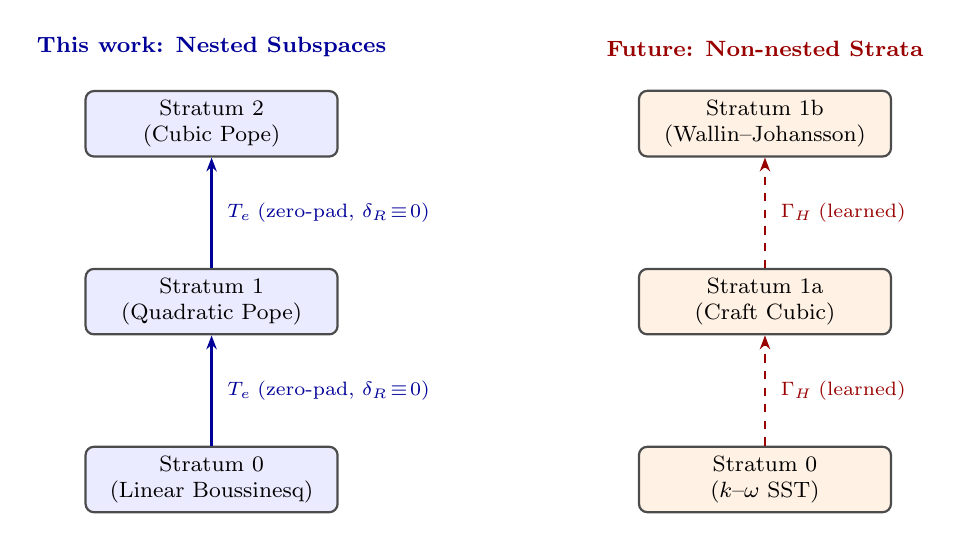
\begin{tikzpicture}[
    node distance=1.4cm and 3.2cm,
    stratum/.style={
      rectangle, rounded corners=3pt, draw=black!70,
      fill=blue!8, minimum width=3.2cm, minimum height=0.7cm,
      font=\footnotesize, align=center, thick
    },
    stratum2/.style={
      rectangle, rounded corners=3pt, draw=black!70,
      fill=orange!10, minimum width=3.2cm, minimum height=0.7cm,
      font=\footnotesize, align=center, thick
    },
    edge_exact/.style={
      -{Stealth[length=5pt]}, thick, blue!60!black
    },
    edge_learned/.style={
      -{Stealth[length=5pt]}, thick, red!60!black, dashed
    },
    label_style/.style={
      font=\scriptsize, midway
    }
  ]
  % --- Vertical: Nested (left column) ---
  \node[stratum] (S0L) {Stratum~0\\(Linear Boussinesq)};
  \node[stratum, above=of S0L] (S1L) {Stratum~1\\(Quadratic Pope)};
  \node[stratum, above=of S1L] (S2L) {Stratum~2\\(Cubic Pope)};

  \draw[edge_exact] (S0L) -- (S1L)
    node[label_style, right=2pt] {$T_e$\;(zero-pad, $\dR\!\equiv\!0$)};
  \draw[edge_exact] (S1L) -- (S2L)
    node[label_style, right=2pt] {$T_e$\;(zero-pad, $\dR\!\equiv\!0$)};

  \node[above=0.3cm of S2L, font=\footnotesize\bfseries, blue!60!black]
    {This work: Nested Subspaces};

  % --- Horizontal: Non-nested (right column) ---
  \node[stratum2, right=3.8cm of S0L] (S0R) {Stratum~0\\($k$--$\omega$ SST)};
  \node[stratum2, above=of S0R] (S1aR) {Stratum~1a\\(Craft Cubic)};
  \node[stratum2, above=of S1aR] (S1bR) {Stratum~1b\\(Wallin--Johansson)};

  \draw[edge_learned] (S0R) -- (S1aR)
    node[label_style, right=2pt] {$\Gamma_H$\;(learned)};
  \draw[edge_learned] (S1aR) -- (S1bR)
    node[label_style, right=2pt] {$\Gamma_H$\;(learned)};

  \node[above=0.3cm of S1bR, font=\footnotesize\bfseries, red!60!black]
    {Future: Non-nested Strata};
\end{tikzpicture}
\caption{Nested vs.\ non-nested structural transitions in the Stratified Design
  Atlas. Vertical transitions (left) are coordinate inclusions where zero-padding
  is exact by construction. Non-nested transitions (right) require learned
  functional transports $\Gamma_H$ and non-convex losses for geometric
  curvature and holonomy to emerge.}\label{fig:horizon}
\end{figure}

The Stratified Design Atlas formalism (Figure~\ref{fig:horizon}) reveals
precisely what ingredients are required for design space geometry to become
non-trivial:
\begin{enumerate}
  \item \textit{Non-nested (horizontal) transitions.} When mutating between
    distinct model families (e.g., swapping timescale formulations or moving
    from $k$-$\epsilon$ to $k$-$\omega$), no coordinate subspace inclusion
    exists. Transport maps must be learned via functional projection (akin to
    continuous knowledge distillation~\cite{Hinton2015}):
    \begin{equation}\label{eq:learned}
      \Gamma_H(\theta_A) = \arg\min_{\theta_B \in \Theta_B}
      \int_\Omega \|\tau_B(\bx;\theta_B) - \tau_A(\bx;\theta_A)\|_F^2\, dA\,.
    \end{equation}
    For linear-in-$\theta$ families, Eq.~(\ref{eq:learned}) reduces to a
    closed-form linear least-squares projection
    $\Gamma_H = G_B^{-1} G_{BA}\, \theta_A$. The round-trip discrepancy
    $\Gamma_{B \to A}(\Gamma_{A \to B}(\theta_A)) - \theta_A$ in that case is
    a linear subspace mismatch defect, not geometric curvature.
  \item \textit{Non-convexity and coupled evaluation.} Genuinely learned
    connections and geometric holonomy require non-convex losses, which arise
    naturally when models are evaluated \emph{a~posteriori} in a coupled
    Navier--Stokes solver, or when nonlinear coefficient neural networks
    $c_n(\bI)$ are introduced. In non-convex multi-basin landscapes, phenomena
    such as mode connectivity, loss barriers, and permutation symmetries~\cite{Draxler2018,Garipov2018,Frankle2018,Ainsworth2022}
    govern path-dependent transitions across disparate local minima.
\end{enumerate}

\subsection{Summary of Contributions}\label{sec:contributions}

\begin{enumerate}
  \item Formalized candidate turbulence closures within a Stratified Design
    Atlas and characterized its simplest instantiation (nested Pope subspaces,
    constant coefficients, convex loss) as an auditable baseline.
  \item Quantified the secondary stress-representability gap for the square
    duct, recovering Speziale's classical result that linear closures produce
    anti-aligned secondary vorticity forcing ($\rho = -0.157$, $29.4\%$ reversed).
  \item Demonstrated that staged calibration inherits scaffold realizability
    violations at deployment ($\delta_R \equiv 0$), while an un-staged cold start
    ($\theta = \mathbf{0}$, Path~C) achieves the lowest peak violation ($1.22\%$)
    throughout the descent.
  \item Disproved the Gram-conditioning instability hypothesis via an ablation
    suite, showing that transient excursions are governed by per-step travel
    distance and adaptive coordinate scaling, with convergent plain GD also
    violating realizability ($6.25\%$), and with per-coordinate Adam restoring
    exact machine-precision scale invariance on normalized bases.
  \item Isolated momentum and travel-distance mechanics via pre-registered controls:
    resetting momentum at matched loss (step~18) yields a post-restart peak of $1.74\%$
    and $3.12\times$ rebound (Branch~ii occurred), confirming that parameter travel
    distance dominates the excursion while momentum provides modest amplification
    ($+0.26\%$), while $\beta_1 = 0$ reduces peak violation to $1.30\%$.
  \item Identified the necessary conditions for design space geometry to become
    non-trivial, providing a concrete roadmap for non-nested model discovery.
\end{enumerate}

% ============================================================================
\begin{acknowledgments}
The authors acknowledge the NumPy, SciPy, and Matplotlib open-source communities.
\end{acknowledgments}
% ============================================================================

\paragraph*{Data and Code Availability.}
All source code, telemetry databases (\texttt{results\_curvature\_experiment.json},
\texttt{results\_audit\_experiments.json}, \texttt{results\_round2\_controls.json}),
and figure scripts are available at
\url{https://github.com/okuhlemadondo/stratified-turbulence-closures}.

\begin{thebibliography}{28}

\bibitem{Ainsworth2022}
  S.~Ainsworth, J.~Hayase, and S.~Srinivasa,
  \emph{Git Re-Basin: Merging Models modulo Permutation Symmetries},
  in \emph{International Conference on Learning Representations (ICLR)} (2023).

\bibitem{Amari1998}
  S.~Amari,
  \emph{Natural Gradient Works Efficiently in Learning},
  Neural Comput.\ \textbf{10}(2), 251--276 (1998).

\bibitem{Ash2020}
  J.~Ash and R.~P.~Adams,
  \emph{On Warm-Starting Neural Network Training},
  in \emph{Advances in Neural Information Processing Systems (NeurIPS)},
  Vol.~33, pp.~3884--3894 (2020).

\bibitem{Bengio2009}
  Y.~Bengio, J.~Louradour, R.~Collobert, and J.~Weston,
  \emph{Curriculum Learning},
  in \emph{International Conference on Machine Learning (ICML)},
  pp.~41--48 (2009).

\bibitem{Boussinesq1877}
  J.~Boussinesq,
  \emph{Essai sur la th\'eorie des eaux courantes},
  M\'emoires pr\'esent\'es par divers savants \`a l'Acad\'emie des Sciences
  de l'Institut National de France \textbf{23}(1), 1--680 (1877).

\bibitem{Chen2016}
  T.~Chen, I.~Goodfellow, and J.~Shlens,
  \emph{Net2Net: Accelerating Learning via Knowledge Transfer},
  in \emph{International Conference on Learning Representations (ICLR)} (2016).

\bibitem{Craft1996}
  T.~J.~Craft, B.~E.~Launder, and K.~Suga,
  \emph{Development and application of a cubic eddy-viscosity model of turbulence},
  Int.\ J.\ Heat Fluid Flow \textbf{17}(2), 108--115 (1996).

\bibitem{Draxler2018}
  F.~Draxler, K.~Veschgini, M.~Salmhofer, and F.~A.~Hamprecht,
  \emph{Essentially No Barriers in Neural Network Energy Landscapes},
  in \emph{International Conference on Machine Learning (ICML)},
  pp.~1309--1318 (2018).

\bibitem{Duraisamy2019}
  K.~Duraisamy, G.~Iaccarino, and H.~Xiao,
  \emph{Turbulence Modeling in the Age of Data},
  Annu.\ Rev.\ Fluid Mech.\ \textbf{51}, 357--377 (2019).

\bibitem{Frankle2018}
  J.~Frankle and M.~Carbin,
  \emph{The Lottery Ticket Hypothesis: Finding Sparse, Trainable Neural Networks},
  in \emph{International Conference on Learning Representations (ICLR)} (2019).

\bibitem{Garipov2018}
  T.~Garipov, P.~Izmailov, D.~Podoprikhin, D.~P.~Vetrov, and A.~G.~Wilson,
  \emph{Loss Surfaces, Mode Connectivity, and Fast Ensembling of DNNs},
  in \emph{Advances in Neural Information Processing Systems (NeurIPS)},
  Vol.~31, pp.~8789--8798 (2018).

\bibitem{Hinton2015}
  G.~Hinton, O.~Vinyals, and J.~Dean,
  \emph{Distilling the Knowledge in a Neural Network},
  arXiv:1503.02531 (2015).

\bibitem{Kochkov2021}
  D.~Kochkov, J.~A.~Smith, A.~Alieva, Q.~Wang, M.~P.~Brenner, and S.~Hoyer,
  \emph{Machine learning-accelerated computational fluid dynamics},
  Proc.\ Natl.\ Acad.\ Sci.\ U.S.A.\ \textbf{118}(21), e2101784118 (2021).

\bibitem{Ling2016}
  J.~Ling, R.~Jones, and J.~Templeton,
  \emph{Machine learning strategies for systems with invariance; application to Reynolds stress closure modelling},
  J.\ Fluid Mech.\ \textbf{807}, 155--166 (2016).

\bibitem{List2022}
  F.~List, L.-W.~Chen, and N.~Thuerey,
  \emph{Learned turbulent field closures with direct numerical simulation data},
  Phys.\ Fluids \textbf{34}(1), 015118 (2022).

\bibitem{Lumley1978}
  J.~L.~Lumley,
  \emph{Computational modeling of turbulent flows},
  Adv.\ Appl.\ Mech.\ \textbf{18}, 123--176 (1978).

\bibitem{Parish2016}
  E.~J.~Parish and K.~Duraisamy,
  \emph{A paradigm for data-driven predictive modeling using field inversion and machine learning},
  J.\ Comput.\ Phys.\ \textbf{305}, 758--774 (2016).

\bibitem{Pinelli2010}
  A.~Pinelli, M.~Uhlmann, A.~Sekimoto, and G.~Kawahara,
  \emph{Reynolds number dependence of mean flow and turbulence statistics in a square duct},
  J.\ Fluid Mech.\ \textbf{644}, 107--122 (2010).

\bibitem{Pope1975}
  S.~B.~Pope,
  \emph{A more general effective-viscosity hypothesis},
  J.\ Fluid Mech.\ \textbf{72}(2), 331--340 (1975).

\bibitem{Pope2000}
  S.~B.~Pope,
  \emph{Turbulent Flows},
  Cambridge University Press (2000).

\bibitem{Prandtl1926}
  L.~Prandtl,
  \emph{\"Uber die ausgebildete Turbulenz},
  Verh.\ 2.\ Int.\ Kongr.\ Tech.\ Mech., Z\"urich, pp.~62--74 (1926).

\bibitem{Schmelzer2020}
  M.~Schmelzer, R.~P.~Dwight, and P.~Cinnella,
  \emph{Discovery of Algebraic Reynolds-Stress Models Using Sparse Symbolic Regression},
  Flow Turbul.\ Combust.\ \textbf{104}, 579--603 (2020).

\bibitem{Schumann1977}
  U.~Schumann,
  \emph{Realizability of Reynolds stress turbulence models},
  Phys.\ Fluids \textbf{20}(5), 721--725 (1977).

\bibitem{Speziale1987}
  C.~G.~Speziale,
  \emph{On nonlinear K-l and K-$\varepsilon$ models of turbulence},
  J.\ Fluid Mech.\ \textbf{178}, 459--475 (1987).

\bibitem{Wallin2000}
  S.~Wallin and A.~V.~Johansson,
  \emph{An explicit algebraic Reynolds stress model for incompressible and compressible turbulent flows},
  J.\ Fluid Mech.\ \textbf{403}, 89--132 (2000).

\bibitem{Weatheritt2016}
  J.~Weatheritt and R.~D.~Sandberg,
  \emph{A novel evolutionary algorithm applied to algebraic Reynolds stress model development},
  J.\ Fluid Mech.\ \textbf{806}, 248--277 (2016).

\bibitem{Wei2016}
  T.~Wei, C.~Wang, Y.~Rui, and C.~W.~Chen,
  \emph{Network Morphism},
  in \emph{International Conference on Machine Learning (ICML)},
  pp.~564--572 (2016).

\bibitem{Wu2018}
  J.-L.~Wu, H.~Xiao, and E.~Paterson,
  \emph{Physics-informed machine learning approach for augmenting turbulence models: A comprehensive framework},
  Phys.\ Rev.\ Fluids \textbf{3}(7), 074602 (2018).

\end{thebibliography}

\end{document}
